\documentclass{article}
\usepackage{amsmath,amssymb,amsfonts}
\usepackage{xcolor}
\usepackage{amsfonts,amsmath}
\usepackage{color}
\usepackage{tikz}
\usetikzlibrary{calc}
\usetikzlibrary{shapes.geometric}
\usetikzlibrary{shapes,decorations,arrows,calc,arrows.meta,fit,positioning}
\tikzset{
	-Latex,auto,node distance =1 cm and 1 cm,semithick,
	state/.style ={ellipse, draw, minimum width = 0.7 cm},
	point/.style = {circle, draw, inner sep=0.04cm,fill,node contents={}},
	bidirected/.style={Latex-Latex,dashed},
	el/.style = {inner sep=2pt, align=left, sloped},
	square/.style={regular polygon,regular polygon sides=4}
}

\newcommand{\myassetnode}[5]{\node[state,circle] (#1) at (#2,#3) {#4};
	\node[state,square,scale=0.5, fill=white!100] (#1asset) at (#2+0.3, #3-0.3) {#5};
}

\begin{document}

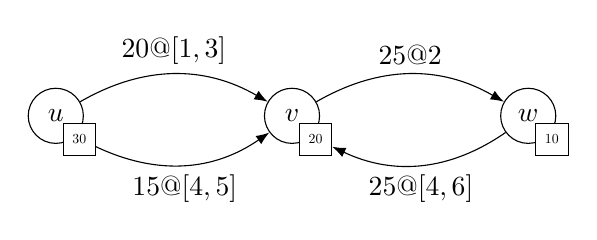
\begin{tikzpicture}
	% the nodes
	\myassetnode{u}{0}{0}{$u$}{$30$}
	\myassetnode{v}{3}{0}{$v$}{$20$}
	\myassetnode{w}{6}{0}{$w$}{$10$}
	% the edges
	\path (u) edge[bend left] node[above] {$20@[1,3]$} (v);
	\path (uasset) edge[bend right] node[below] {$15@[4,5]$} (v);
	\path (v) edge[bend left] node[above] {$25@2$} (w);
	\path (w) edge[bend left] node[below] {$25@[4,6]$} (vasset);
\end{tikzpicture}

\end{document}